\begin{definition}
    The \emph{break-even points} are the points at which total revenue = total cost.
\end{definition}

A profit is made when \(total \ revenue > total \ cost.\) If the sale of a product changes from a profit to a loss or vice versa at some quantity \(q,\) then this occurred at a break-even point.

\begin{image}
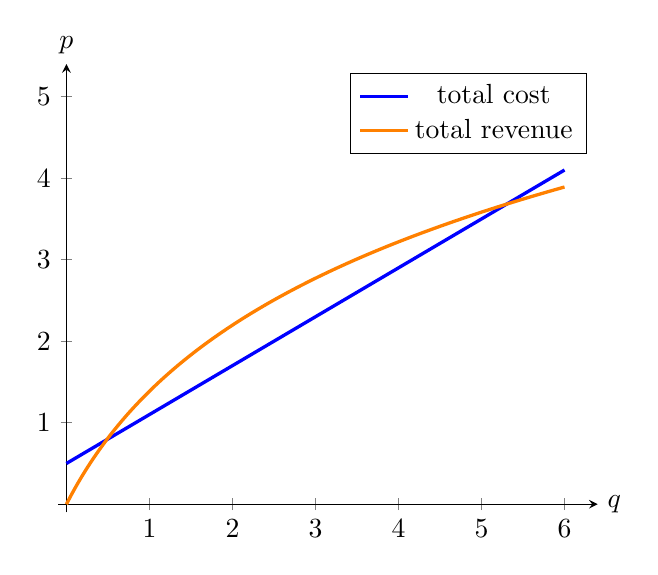
\begin{tikzpicture}
  \begin{axis}[
  xmin=-0.1,
  xmax=6.4,
  ymin=-.1,
  ymax=5.4,
  axis lines=center,
  xlabel=$q$,
  ylabel=$p$,
  every axis y label/.style=
    {at=(current axis.above origin),anchor=south},
  every axis x label/.style=
    {at=(current axis.right of origin),anchor=west},
  ]
\addplot [very thick, blue, smooth, samples=100, domain=0:6] {0.6*x+0.5};
\addlegendentry{total cost}
\addplot [very thick, orange, smooth, samples=100, domain=0:6] {2*ln(x+1)};
\addlegendentry{total revenue}
\end{axis}
\end{tikzpicture}
\end{image}

Note that we have two break-even points for the above product. One that occurs at a price of about \(0.8\) and another that is happening at a price of about \(3.7.\) Between these two prices we have a profit since \(total \ revenue > total \ cost.\) At prices outside of this window, we have a loss. We remark that calculus is exactly constructed to answer the question ``At what price is total profit maximal?'' Calculus is an excellent tool for finding maximums and minimums. With algebra only, we are equipped to find maximum and minimum values for quadratics, but not much else.